\documentclass{ximera}

\usepackage{float}

\newcommand{\R}{\mathbb R}

\newcommand{\href}[2]{#2\footnote{\url{#1}}}
\newcommand{\verticalvector}[1]{\begin{bmatrix}#1\end{bmatrix}}
\newcommand{\gt}{>}

\pgfplotsset{compat=1.8}
\graphicspath{
{./}
{introduction/}
{unit1/}
{unit1/theGeometryOfLinearEquations/}
{unit1/EliminationwithMatrices/}
{unit1/MultiplicationandInverseMatrices/}
}


\title{Elimination with matrices}

\begin{document}
\begin{abstract}
  Unit 1 MIT OCW Linear Algebra: Elimination with matrices
\end{abstract}
\maketitle

The MIT OCW Video Lecture can be found
here:\video{https://www.youtube.com/watch?v=QVKj3LADCnA}

This session introduces the method of elimination, an essential tool for working 
with matrices. The method follows a simple algorithm. To help make sense of material 
presented later, we describe this algorithm in terms of matrix multiplication.

\begin{figure}[H]
\begin{image}
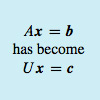
\includegraphics{1_2.jpg}
\end{image}
\end{figure}

\section*{Method of Elimination}

\[A = \begin{bmatrix} 1&2&1\\3&8&1\\0&4&1 \end{bmatrix}\]and\[\mathbf{b} = \verticalvector{2\\12\\2}\]


The number $1$ in the upper left corner of $A$ is called the first pivot. We 
recopy the first row, then multiply the numbers in it by an appropriate value 
(in this case $3$) and subtract those values from the numbers in the second row.
The first number in the second row becomes $0$. We have thus eliminated the $3$ 
in row $2$ column $1$.

The next step is to perform another elimination to get a $0$ in row $3$ column $1$; 
here this is already the case.

The second pivot is the value $2$ which now appears in row $2$ column $2$. 
We find a multiplier (in this case $2$) by which we multiply the second row to 
eliminate the $4$ in row $3$ column $2$. The third pivot is then the $5$ 
now in row $3$ column $3$.

We started with an invertible matrix $A$ and ended with an upper triangular matrix $U$;
the lower left portion of U is filled with zeros. Pivots 1, 2, 5 are on the diagonal
of $U$.

\[A = \begin{bmatrix} 1&2&1\\3&8&1\\0&4&1 \end{bmatrix} \longrightarrow
\begin{bmatrix} 1&2&\phantom{-} 1\\0&2&-2\\0&4&\phantom{-} 1 \end{bmatrix} 
\longrightarrow U = \begin{bmatrix} 1&2&\phantom{-}1\\0&2&-2\\0&0&\phantom{-}5 \end{bmatrix} 
\]

We repeat the multiplications and subtractions with the vector $B = \verticalvector{2\\12\\2}$

For example, we multiply the $2$ in the first position by $3$ and subtract from $12$
to get $6$ in the second position. When calculating by hand we can do this efficiently
by augmenting the matrix $A$, appending the vector $b$ as a fourth or final column. 
The method of elimination transforms the equation $A\mathbf{x} = \mathbf{b}$ 
into a new equation $U\mathbf{x} = \mathbf{c}$. In the example above 
$U = \begin{bmatrix} 1&2&\phantom{-}1\\0&2&-2\\0&0&\phantom{-}5 \end{bmatrix}$
comes from $A$ and $c=\verticalvector{\phantom{-}2\\\phantom{-}6\\-10}$ comes from 
$\mathbf{b}$.

The equation $U\mathbf{x} = \mathbf{c}$ is easy to solve by back substitution; 
in our example, $z = -2$, $y = 1$ and $x = 2$. This is also a solution to the 
original system $A\mathbf{x} = \mathbf{b}$.

The determinant of $U$ is the product of the pivots. We will see this again.

Pivots may not be $0$. If there is a zero in the pivot position, we must exchange 
that row with one below to get a non-zero value in the pivot position. 

If there is a zero in the pivot position and no non-zero value below it, 
then the matrix $A$ is not invertible. Elimination can not be used to find a 
unique solution to the system of equations as it doesnt exist.

\section*{Elimination Matrices}

The product of a matrix $(3x3)$ and a column vector $(3x1)$ is a column vector 
$(3x1)$ that is a linear combination of the columns of the matrix.

The product of a row $(1x3)$ and a matrix $(3x3)$ is a row $(1x3)$ that is a linear
combination of the rows of the matrix.

We can subtract $3$ times row $1$ of matrix $A$ from row $2$ of $A$ by calculating 
the matrix product:

\[
\begin{bmatrix} \phantom{-}1&0&0\\-3&1&0\\\phantom{-}0&0&1 \end{bmatrix}
\cdot 
\begin{bmatrix} 1&2&1\\3&8&1\\0&4&1 \end{bmatrix} =
\begin{bmatrix} 1&2&\phantom{-}1\\0&2&-2\\0&4&\phantom{-}1 \end{bmatrix}
\]

The elimination matrix used to eliminate the entry in row m column n is denoted $E_{mn}$. 
The calculation above took us from $A$ to $E_{21}A$. The three elimination steps 
leading to $U$ were: $E_{32}(E_{31}(E_{21}A)) = U$, where $E_{31} = I$. Thus 
$E_{32}(E_{21}A) = U$.

Matrix multiplication is associative, so we can also write $(E_{32}E_{21})A = U$. 
The product $E_{32}E_{21}$ tells us how to get from $A$ to $U$. The inverse of the matrix 
$E_{32}E_{21}$ tells us how to get from $U$ to $A$.

If we solve $U\mathbf{x} = EA\mathbf{x} = E\mathbf{b}$, then it is also true that 
$A\mathbf{x} = \mathbf{b}$. This is why the method of elimination works: all steps 
can be reversed.

A permutation matrix exchanges two rows of a matrix; for example,

\[
P=\begin{bmatrix} 0&1&0\\1&0&0\\0&0&1 \end{bmatrix}
\]

The first and second rows of the matrix $PA$ are the second and first rows of the 
matrix $A$. The matrix $P$ is constructed by exchanging rows of the identity matrix.

To exchange the columns of a matrix, multiply on the right (as in $AP$) by a 
permutation matrix.

Note that matrix multiplication is not commutative: $PA \neq AP$.

\section*{Inverses}

We have a matrix:

\[
 E_{21} = \begin{bmatrix} \phantom{-}0&1&0\\-3&1&0\\\phantom{-}0&0&1 \end{bmatrix}
\]

which subtracts 3 times row 1 from row 2. To undo this operation we must add 3 times 
row 1 to row 2 using the inverse matrix:

\[
 E_{21}^{-1} = \begin{bmatrix} 0&1&0\\3&1&0\\0&0&1 \end{bmatrix}
\]


In fact, $ E_{21}^{-1}E_{21} = I$.

\section*{Recitation}

\begin{question}
Today's problem is a straightforward solve the following linear system with four 
equations and four unknowns, using the method of elimination. The system is 
\begin{align*}
  x  - y -    z + u  =  0\\
2x        +2z         =  8\\
      - y  - 2z         = -8\\
3x -3y - 2z + 4u =  7\\
\end{align*}
And although you might know different ways to solve the system at this point,
the method of elimination is going to show up a million times during these videos,
so it's really important to get it right.
\begin{solution}
\begin{hint}
So the method of elimination, if you remember it from class, consisted of replacing
this system with an equivalent system-- equivalent meaning they have the same solution--
by a series of row operations. Row operations are not supposed to change the solution 
to the system and there, for example, exchange the order of two equations. 
Multiply an equation with a non-0 number, and add a non-0 multiple of one equation 
to the other. So let's do that.

As we're going to do this series of arithmetic operations, we don't really want
to copy the names of the variables and the equality signs every time. So we're
going to keep the important information which are these numbers. these coefficients
here, we're going to keep that information in a matrix.
So let's write a matrix. Each row is going to grasp onto an equation, and each column
is going to correspond to an unknown.

\begin{matrixAnswer}[name=M]
      The matrix is  [['1','-1','-1','1','0'],['2', '0','2','0','8'],
      	['0','-1','-2','0','-8'],['0','-3','-2',4','7']]
 \end{matrixAnswer}

\end{hint}
\begin{hint}
OK, and now let's try reducing this matrix to an upper triangular one. We start with
the first column, and we're going to use this number called a pivot to get rid of all
the numbers under it, so to get 0s here and here. A way to do it is-- well, to get rid
of this 2, I have to multiply the first row by -2, and add it to the second one. The
third row already has a 0 in the first column so no change. Multiply the first row by
-3 and add it to the fourth row.

\begin{matrixAnswer}[name=M]
      The matrix is  [['1','-1','-1','1','0'],['0', '2','4','-2','8'],
      ['0','-1','-2','0','-8'],['0','0,'1',1','7']]
 \end{matrixAnswer}
\end{hint}
\begin{hint}
The first column looks like a first column of an upper triangular matrix. Now let's
do the same to the second column. This is going to be our pivot, the number that we
use to get rid of numbers under it. And we see that to get rid of this number here,
we will need to multiply it with 1/2. So multiply the whole second row with 1/2, and
add it to the third row. The fourth row already has a zero in this column.
\begin{matrixAnswer}[name=M]
      The matrix is  [['1','-1','-1','1','0'],['0', '2','4','-2','8'],
      ['0','0','0','-1','-4'],['0','0,'1',1','7']]
 \end{matrixAnswer}
And now let's look at this matrix. It has the first two columns as they're supposed
to be, 0s under the diagonal. 
\end{hint}

\begin{hint}
You might remember from lecture that 0s can never be pivots. Or you can just try
finding a number such that 0 times this number equals -1, and seeing that such a
number doesn't exist, because you're always going to get 0.

But is there another way to get a 0 here? There is a very simple row operation,
which consists just of switching the third and the fourth row. It certainly doesn't
change the solution of the system. 
\begin{matrixAnswer}[name=M]
      The matrix is  [['1','-1','-1','1','0'],['0', '2','4','-2','8'],
      ['0','0,'1',1','7'],['0','0','0','-1','-4']]
\end{matrixAnswer}
\end{hint}

\begin{hint}
So in the same way as at the beginning, we had a system and then wrote the matrix
representing it, this matrix also represents a system. And this system has the same
solutions as the initial system but is much easier to solve. Now let's write this
back as a system, and let me do that not starting from the first equation, but
starting from the last equation. So the last equation here reads -u equals -4, which
is, as equations go, a pretty easy one to solve. The solution is u equals 4.\end{hint}
\begin{align*}
-u  =  4\\
z+u=7\\
2y+4z-2u=8\\
x-y-z+u=0\\
\end{align*}
$x = \answer{1}$\\
$y = \answer{2}$\\
$z = \answer{3}$\\
$u = \answer{4}$\\


This finishes the problem, but I would very strongly encourage you now to take this
solution and plug it back into the original system and check if it's really a solution.

\end{solution}
\end{question}


The MIT Recitation video for this question is here:
here:\video{https://www.youtube.com/watch?v=xCIXkm3-ocQ}

\section*{Homework}

\begin{question}

In the two-by-two system of linear equations below, what multiple of the first
equation should be subtracted from the second equa�tion when using the method of
elimination? Convert this system of equa�tions to matrix form, apply elimination
(what are the pivots?), and use back substitution to find a solution. Try to check
your work before look�ing up the answer.
\begin{align*}
2x + 3y = 5 \\
6x + 15y = 12
\end{align*}

\begin{solution}
\begin{hint}
\begin{matrixAnswer}[name=M]
      The matrix is  [['2','3','5'],['6','15','12']]
\end{matrixAnswer}
\end{hint}

\begin{hint}
We then apply elimination on matrix A. Using the first pivot (the num�ber 2 in the upper
left corner of A), we subtract three times the first row from the second row
\begin{matrixAnswer}[name=M]
      The matrix is  [['2','3','5'],['0','6','-3']]
\end{matrixAnswer}
\end{hint}
\begin{hint}
\begin{align*}
6y=-3 \rightarrow y=-\frac{1}{2}\\
2x + 3y=5 \rightarrow 2x + 3 \cdot (-\frac {1}{2}) = 5 \rightarrow x = \frac {13}{4}\\
\end{align*}
\end{hint}
$x =  \answer{\frac {13}{4}}$\\
$y = \answer{-\frac {1} {2}}$
\end{solution}
\end{question}

\begin{question}
(2.3 29. Introduction to Linear Algebra: Strang) Find the triangular matrix E
that reduces "Pascal's matrix" to a smaller Pascal
\begin{align*}
E \begin{bmatrix} 1&0&0&0\\1&1&0&0\\1&2&1&0\\1&3&3&1 \end{bmatrix} =
\begin{bmatrix} 1&0&0&0\\0&1&0&0\\0&1&1&0\\0&1&2&1 \end{bmatrix}
\end{align*}
Which matrix M (multiplying several E's) reduces Pascal all the way to I?

\begin{solution}
\begin{hint}
\end{hint}
\begin{matrixAnswer} [name=M] 
M = [ ['1','0','0','0'], ['-1','1','0','0'], ['1','-2','1','0'], ['-1','3','-3','1']]
\end{matrixAnswer}

\end{solution}
\end{question}

\end{document}
